\documentclass[11pt,letterpaper]{article}
\usepackage[margin=.72in]{geometry}
\usepackage[T1]{fontenc}
\usepackage{lmodern,microtype,booktabs,array,graphicx,pdflscape,xcolor,amsmath,hyperref}
\hypersetup{colorlinks=true,urlcolor=blue,linkcolor=blue,pdftitle={Arrival-delay labels at the minute boundary}}
\setlength{\parindent}{0pt}\setlength{\parskip}{6pt}
\newcommand{\heading}[1]{\vspace{4pt}{\large\bfseries #1}\par}
\newcommand{\BoundA}{275}
\newcommand{\BoundB}{44,707}
\newcommand{\BoundC}{131}
\newcommand{\BoundD}{18,805}
\newcommand{\BoundE}{0.697}
\newcommand{\BoundF}{144}
\newcommand{\BoundG}{25,902}
\newcommand{\BoundH}{0.556}
\newcommand{\BoundI}{547,271}
\newcommand{\BoundJ}{46,621}
\newcommand{\BoundK}{21,303}
\newcommand{\BoundL}{20,327}
\newcommand{\BoundM}{26,294}
\newcommand{\BoundN}{18,805}
\newcommand{\BoundO}{25,902}
\newcommand{\BoundP}{0}
\newcommand{\BoundQ}{0}
\newcommand{\BoundR}{0}
\newcommand{\BoundS}{0}
\newcommand{\BoundT}{0}
\newcommand{\BoundU}{0}
\newcommand{\BoundV}{0}
\newcommand{\BoundW}{0}
\newcommand{\BoundX}{1,479}
\newcommand{\BoundY}{311}
\newcommand{\BoundZ}{43}
\newcommand{\BoundAA}{81}
\newcommand{\BoundAB}{0}
\newcommand{\BoundAC}{0}
\newcommand{\BoundAD}{18,805}
\newcommand{\BoundAE}{25,902}
\newcommand{\BoundAF}{0}
\newcommand{\BoundAG}{0}
\newcommand{\BoundAH}{0}
\newcommand{\BoundAI}{0}
\newcommand{\BoundAJ}{5,122}
\newcommand{\BoundAK}{5,571}
\newcommand{\BoundAL}{27.24}
\newcommand{\BoundAM}{21.51}
\newcommand{\BoundAN}{4,989}
\newcommand{\BoundAO}{5,377}
\newcommand{\BoundAP}{26.53}
\newcommand{\BoundAQ}{20.76}
\newcommand{\BoundAR}{4,858}
\newcommand{\BoundAS}{5,233}
\newcommand{\BoundAT}{25.83}
\newcommand{\BoundAU}{20.20}
\newcommand{\BoundAV}{2.63}
\newcommand{\BoundAW}{2.68}
\newcommand{\BoundAX}{62}
\newcommand{\BoundAY}{26}
\newcommand{\BoundAZ}{270}
\newcommand{\BoundBA}{131,867}
\newcommand{\BoundBB}{191,424}
\newcommand{\BoundBC}{2,947}
\newcommand{\BoundBD}{26}
\newcommand{\BoundBE}{29}
\newcommand{\BoundBF}{3.10.11}
\newcommand{\BoundBG}{3.12.14}
\newcommand{\BoundBH}{6}
\newcommand{\BoundBI}{10}
\newcommand{\BoundBJ}{90}
\newcommand{\BoundBK}{360}
\begin{document}
{\LARGE\bfseries Arrival-delay labels at the minute boundary\par}
\vspace{5pt}
Independent research program\hfill 31 October 2026 UTC\\
\textit{Not peer reviewed. One current source view; fixed recorded-minute probes.}

\heading{Practical finding}
Changing a delay cutoff changes the target even when the flights stay the same. In the fixed January 2024 reporting-carrier cohort, \BoundA{} of \BoundB{} eligible records change labels between recorded cutoffs of 15 and 16 minutes.

At ORD the affected count is \BoundC{} of \BoundD{}, a \BoundE{} percentage-point rate difference. At ATL it is \BoundF{} of \BoundG{}, or \BoundH{} percentage points. These are sensitivity results on recorded minutes, not a reconstruction of a European rate or physical-second lateness.

\heading{Recommended use}
Keep the source field, numeric cutoff and eligible denominator with a benchmark label. Rebuild the label from supported source observations before pooling systems. Retain cancellation, diversion and unknown-field accounts alongside completed-flight rates. A matching label name or published aggregate is insufficient evidence that the target and population match.

The local implementation returns qualified recorded-minute counts and rejects unsupported requests to infer physical seconds, European OTP15, safety rankings or a transfer score. This is a runnable implementation exercise, not a deployed forecasting service or measured operating benefit.

\heading{Source and fixed scope}
The official BTS January 2024 reporting-carrier archive contains \BoundI{} national rows. Every arrival to the two fixed destination codes is retained: \BoundJ{} records in \BoundK{} day/carrier/source-state count cells. Native archives and flight identities remain private.

The public protocol fixed month, destinations, eligibility and cutoffs before flight-record retrieval. After the source form failed, the official archive directory supplied a published direct link to the identical fixed file. That transport change was committed before reading its body. The earlier failure is preserved; no month, airport or reporting-population substitution was made.

\heading{Original transfer question remains unexecuted}
The original US-to-Europe model-transfer study remains unexecuted. Common-event, reporting-population, source-rights and historical-vintage requirements remain unresolved. The 16-minute probe is an authored comparison on US recorded values. It does not equate US minutes with European physical-second labels. No European source values are transformed or scored.
\newpage
{\Large\bfseries Complete airport accounts and denominators\par}
The rate denominator contains eligible completed nondiverted source records. Negative early arrivals remain eligible. The early-arrival-clamped field was not substituted. Missing or malformed values remain explicit.

{\small\setlength{\tabcolsep}{7pt}
\begin{tabular}{@{}lrr@{}}\toprule
Source account & ORD & ATL\\\midrule
All selected source records & \BoundL{} & \BoundM{} \\
Eligible completed nondiverted & \BoundN{} & \BoundO{} \\
Missing key & \BoundP{} & \BoundQ{} \\
Duplicate key & \BoundR{} & \BoundS{} \\
Unknown operation flags & \BoundT{} & \BoundU{} \\
Both operation flags set & \BoundV{} & \BoundW{} \\
Cancelled & \BoundX{} & \BoundY{} \\
Diverted & \BoundZ{} & \BoundAA{} \\
Unknown delay & \BoundAB{} & \BoundAC{} \\
Usable official indicator among eligible & \BoundAD{} & \BoundAE{} \\
Unknown official indicator among eligible & \BoundAF{} & \BoundAG{} \\
Official indicator mismatch among eligible & \BoundAH{} & \BoundAI{} \\
\bottomrule\end{tabular}}

\heading{All fixed recorded-minute thresholds}
{\small\setlength{\tabcolsep}{7pt}
\begin{tabular}{@{}llrr@{}}\toprule
Cutoff & Quantity & ORD & ATL\\\midrule
Recorded delay >= 14 & Positive count & \BoundAJ{} & \BoundAK{} \\
 & Percent of eligible & \BoundAL{}\% & \BoundAM{}\% \\
Recorded delay >= 15 & Positive count & \BoundAN{} & \BoundAO{} \\
 & Percent of eligible & \BoundAP{}\% & \BoundAQ{}\% \\
Recorded delay >= 16 & Positive count & \BoundAR{} & \BoundAS{} \\
 & Percent of eligible & \BoundAT{}\% & \BoundAU{}\% \\
\bottomrule\end{tabular}}

Fifteen follows the source indicator definition; 14 and 16 are prespecified one-minute probes, not optimized replacements. The primary rate difference is the exact recorded bin $15 \leq \text{ArrDelay}<16$ divided by the eligible count. As a share of the recorded >=15 positives, that bin is \BoundAV{}\% at ORD and \BoundAW{}\% at ATL. A zero denominator is unavailable, never silently zero.

\heading{Complete case retention}
The repository exports all \BoundAX{} airport-day accounts, \BoundAY{} airport/carrier accounts and \BoundAZ{} threshold cases. Every day is retained. The carrier grid includes zero-row combinations with unavailable rates and all source code labels; it does not rank carrier quality. Agreement with the source indicator in this finite cohort does not establish general source accuracy, physical seconds or cross-system equivalence.
\newpage
{\Large\bfseries Verification, implementation and next evidence\par}

\heading{Independent evidence}
A separate pandas C parser, SQLite key classification and exact Fraction values reconcile the captured native source in \BoundBA{} finite conditions. Saved native-bound source checks pass \BoundBB{}. An independent weighted SQLite/Fraction checker reconstructs all accounts, thresholds, numerators, denominators and example requests in \BoundBC{} conditions without importing the production metric functions.

The committed freeze binds \BoundBD{} actual source/method dependencies before threshold comparisons. Source values were visible during capture and reconciliation; this was source informed, not blinded. The \BoundBE{} authored fixture methods cover exact cutoff and fractional-minute values, negative delay, unknown fields, operation flags, duplicate groups, zero denominators, indicator disagreement and unsupported interpretations.

Separate full-history CPython \BoundBF{} and \BoundBG{} replays reproduce \BoundBH{} result files exactly, preserving \BoundBI{} source-directory files in each. Figure checks bind \BoundBJ{} bars and \BoundBK{} actual SVG coordinate conditions. These finite checks are not universal correctness guarantees.

\heading{Runnable implementation exercise}
Seven complete requests accept two qualified recorded-minute rate descriptions and reject five unsupported requests. The interface retains the actual numerator, eligible denominator and exact ratio, plus explicit unknown physical-second and European equivalence. It checks supplied verified accounts; it does not certify arbitrary caller input.

\begin{verbatim}
python -m pip install -r requirements.txt
python src/replay.py --out ../arrival-label-replay
\end{verbatim}
Use a new output directory. The replay checks frozen saved source counts; it does not reacquire the archive or establish original publication timing.

\heading{Material limits}
One winter month, two destination codes and one reporting-carrier source form a convenience cohort. Current historical data can be revised, and the dataset is not an immutable original-vintage capture. Recorded-minute values do not recover the physical-second distribution. No cross-region calibration, causal airport effect, carrier safety/quality score, new estimator, production deployment or realized saving is claimed.

A transfer follow-up needs threshold-resolved compatible targets, aligned operated/cancelled populations, suitable source rights and verified dated availability. Formal-publication projects, including Azure optimization, remain private. Public artifacts contain minimal federal statistical counts and original analysis; native flight identities, tail numbers and source files remain private.

{\small Source: U.S. Department of Transportation, Bureau of Transportation Statistics.
\url{https://transtats.bts.gov/PREZIP/}.
Official field definitions, exact indexed archive URL, capture/member hashes and failed-form history are retained in the repository. This independent study is not endorsed by DOT/BTS. MIT covers original code; source facts are attributed separately.}
\begin{landscape}
{\large\bfseries Recorded threshold rates\par}
\begin{center}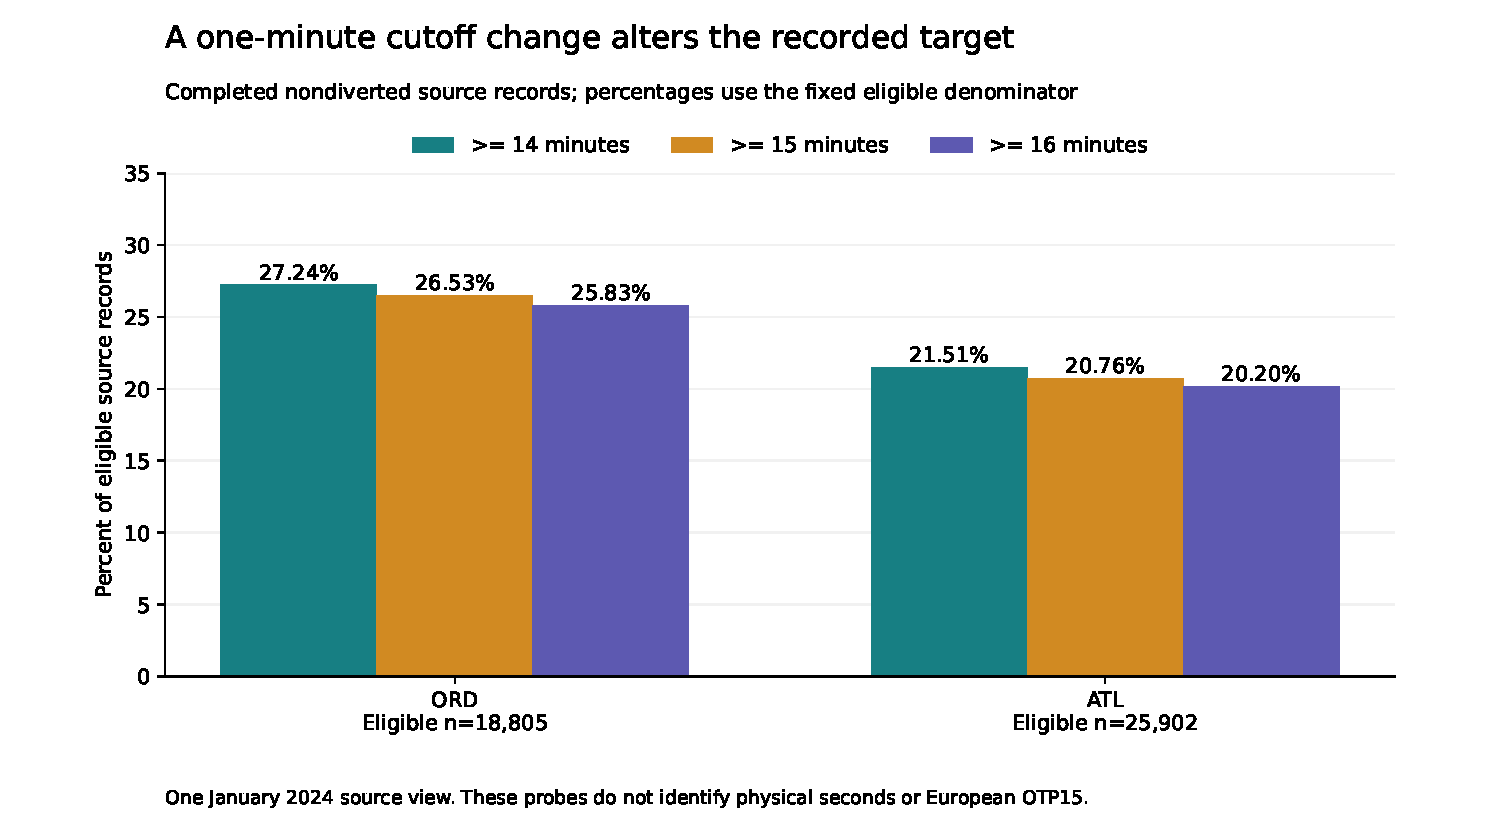
\includegraphics[width=9.4in,height=6.25in,keepaspectratio]{images/threshold_rates.pdf}\end{center}
\end{landscape}
\begin{landscape}
{\large\bfseries Every fixed source day\par}
\begin{center}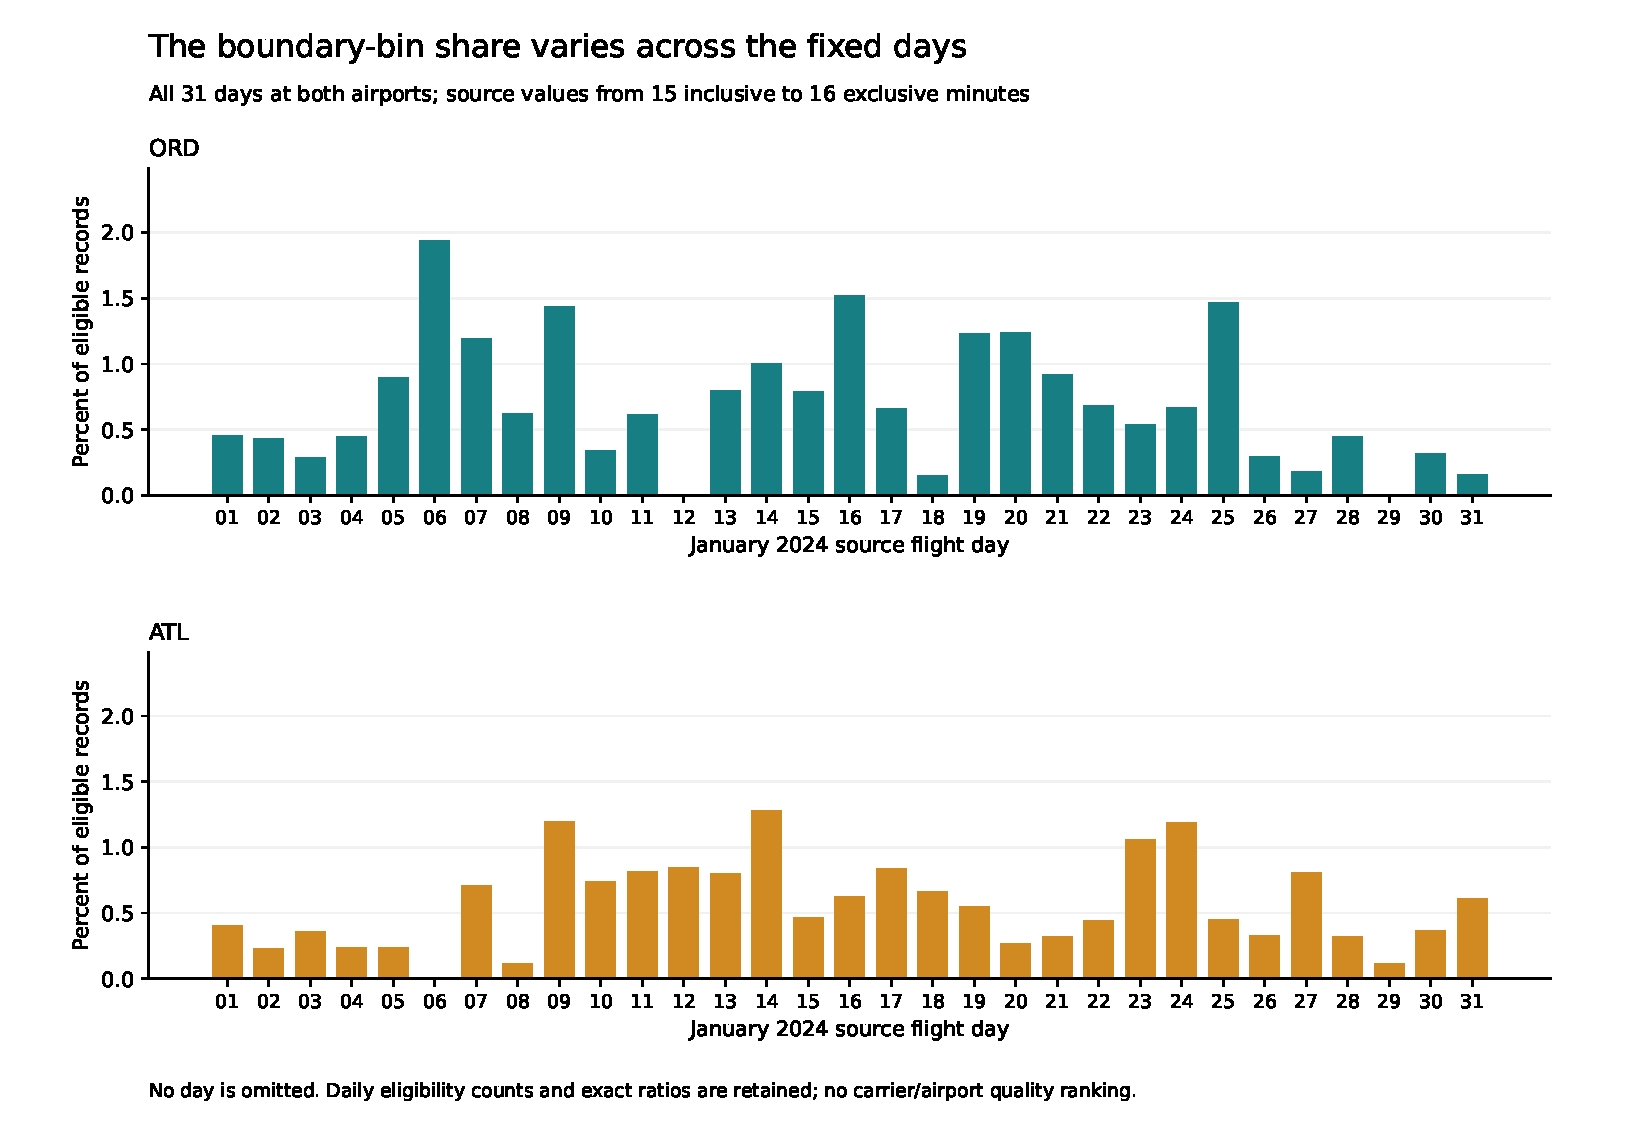
\includegraphics[width=9.4in,height=6.25in,keepaspectratio]{images/daily_boundary.pdf}\end{center}
\end{landscape}
\begin{landscape}
{\large\bfseries Source eligibility and indicator reconciliation\par}
\begin{center}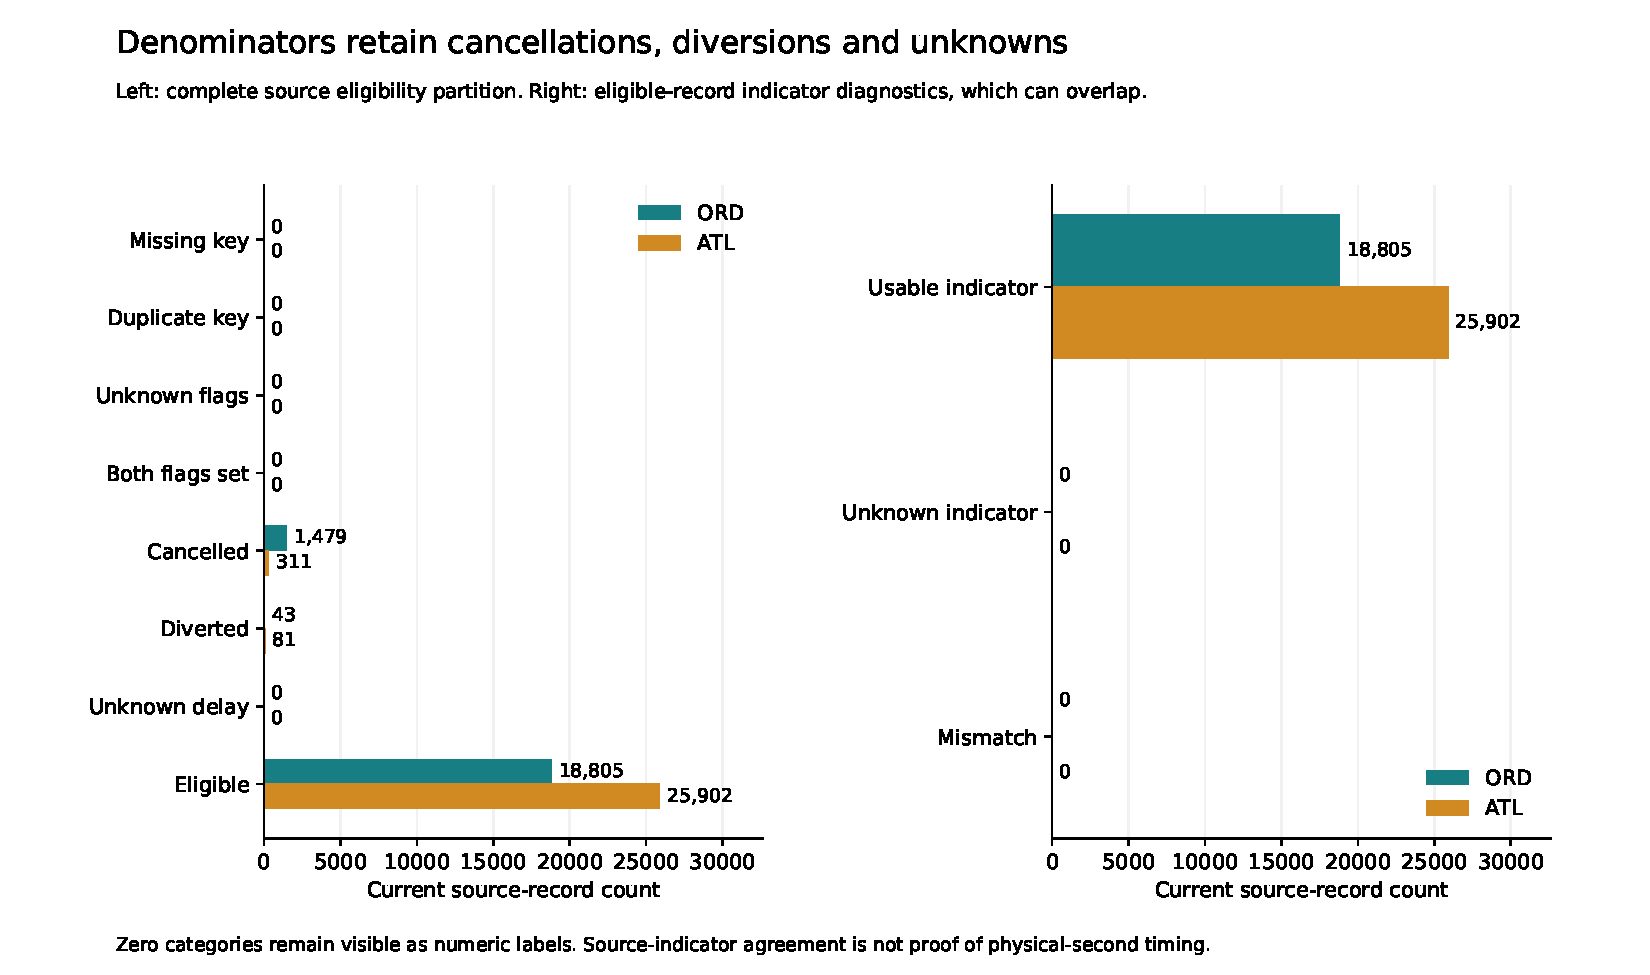
\includegraphics[width=9.4in,height=6.25in,keepaspectratio]{images/source_denominators.pdf}\end{center}
\end{landscape}
\end{document}
